\documentclass[twocolumn,oneside,a4paper]{article}
\title{極座標ステージとエクストルーダの同期に関する考察}
\author{青木 翔平}

\usepackage[usenames]{color} %used for font color
\usepackage{amssymb} %maths
\usepackage{amsmath,cases}
\usepackage{amssymb}
\usepackage{mathrsfs}
\usepackage{multirow}
\usepackage{itembkbx}
\usepackage{graphicx}
\usepackage[utf8]{inputenc} %useful to type directly diacritic characters
%\usepackage{algorithm}
\usepackage{algorithmic}
\usepackage{capt-of}
\usepackage{framed}
%\usepackage[boxed,linesnumbered,figure]{algorithm2e}
\usepackage[ruled,vlined]{algorithm2e}
\usepackage{ascmac}
\usepackage[titletoc,title]{appendix}
\usepackage{bm}
\usepackage{relsize}
\renewcommand{\sectionmark}[1]{\markleft{\thesection\ #1}}
\newcommand\scalemath[2]{\scalebox{#1}{\mbox{\ensuremath{\displaystyle #2}}}}
\usepackage{booktabs} \newcommand{\ra}[1]{\renewcommand{\arraystretch}{#1}}
\let\oldbibliography\thebibliography
\renewcommand{\thebibliography}[1]{\oldbibliography{#1}
\setlength{\itemsep}{0pt}} %Reducing spacing in the bibliography.
\usepackage{mathtools, cuted}
\usepackage{lastpage}
\usepackage{fancyhdr}
 \pagestyle{fancy}
%\lhead{線速度問題の解決}
%\lhead{\leftmark}
\lhead{極座標ステージとエクストルーダの同期に関する考察}
\rhead{[\ \scshape\oldstylenums{\thepage}\ / %
    \scshape\oldstylenums{\pageref{LastPage}}\ ]}
 \rfoot{\copyright \hspace{0.001in} 2016. Keio University}
 
\setlength{\oddsidemargin}{0.1cm}
\setlength{\evensidemargin}{0.1cm}
\setlength{\textwidth}{50zw}

\newcommand\inlineeqno{\stepcounter{equation}\ (\theequation)}

\begin{document}
\maketitle

\section{ステージ側の線速度について}
極座標におけるステージ側の線速度を一定にできるかという問題について,理論的な検討を行う.

デカルト座標系での線速度$v$は極座標で以下のように表される.
\begin{eqnarray}
|v| &=& \sqrt{\dot{x}^2 + \dot{y}^2} \nonumber \\
  &=& \sqrt{ \left(\frac{d}{dt} r \cos\theta \right) ^2 + \left(\frac{d}{dt}r \sin\theta\right) ^2} \nonumber \\
  &=& \sqrt{ \dot{r}^2+ r^2 \dot{\theta}^2 }
\end{eqnarray}    
    
いま,角速度と半径方向の速度を制御して線速度一定にすることを考える.
$v=k$(線速度一定)とすると,
\begin{eqnarray}\label{eq:vdef}
  \dot{r}^2+ r^2 \dot{\theta}^2 &=& k^2 \\
  \dot{r}^2 &=&  k^2 - r^2 \dot{\theta}^2
\end{eqnarray}
微小区間で考えると

\begin{eqnarray}\label{eq:deltar}
     \left( \frac{\Delta r}{\Delta t}\right)^2 &=&  k^2 - r^2 \left( \frac{\Delta \theta}{\Delta t}\right)^2 \nonumber \\
|\Delta r| &=& \sqrt{(k \Delta t)^2 - (r \Delta \theta)^2}
\end{eqnarray}

いっぽう,NCコードにおいて直線移動命令G1が与えられたとき,CNCコントローラではブレゼンハムのアルゴリズム(Algorithm \ref{alg:bresenham})にしたがって補間位置$\{x_1,x_2,...,x_n\},\{y_1,y_2,...,y_n\}$が計算される.
また,計算された$\{x_1,x_2,...,xw_n\},\{y_1,y_2,...,y_n\}$は以下の関係式を用いて$\{r_1,r_2,...,r_n\},\{\theta_1,\theta_2,...,\theta_n\}$へと座標変換される. 
\begin{eqnarray*}
\left\{
  \begin{array}{ll}
r_i = \sqrt{{x_i}^2+{y_i}^2} \\    
\theta_i = \tan^{-1} (y_i / x_i)
  \end{array}
  \right.
\end{eqnarray*}
すなわち,差分形式とすれば
\begin{eqnarray}\label{eq:diff}
\left\{
  \begin{array}{ll}
\Delta r = r_2-r_1 = \sqrt{{x_2}^2+{y_2}^2} - \sqrt{{x_1}^2+{y_1}^2} \\    
\Delta \theta = \theta_2-\theta_1 = \tan^{-1} (y_2 / x_2) - \tan^{-1} (y_1 / x_1)
  \end{array}
  \right.
\end{eqnarray}

一般に,(\ref{eq:diff})で指定される$\Delta r, \Delta \theta$が(\ref{eq:deltar})式を満たすとは限らないため\footnote{$r$の自由度が残る.},任意の目的地の座標が指定されたときに線速度を一定にすることはできない.
%\newpage

\begin{algorithm}                 
\begin{algorithmic}                 
\label{alg:bresenham}                         
\STATE $dx \Leftarrow x1-x0$
\STATE $dy \Leftarrow y1-y0$
\STATE $D \Leftarrow 2*dy - dx$
\STATE plot(x0,y0)
\STATE $y \Leftarrow y0$
\FOR{$x$ from $x0+1$ to $x1$}
\IF{$D > 0$}
\STATE      $y \Leftarrow y+1$
\STATE      plot(x,y)
\STATE      $D \Leftarrow D + (2*dy-2*dx)$
\ELSE
\STATE      plot(x,y)
\STATE      $D \Leftarrow D + (2*dy)$
\ENDIF
\ENDFOR
\end{algorithmic}
\caption{Interpolation of Bresenham}
\end{algorithm}

\section{エクストルーダの制御について}
%\vspace{0.2in}
ステージの変位と射出量の関係について考える.

デカルト座標系において,移動時間$\Delta t$と線速度$F$[mm/min]の関係は,以下のように表される.

\begin{eqnarray}
     \Delta t = \frac{\sqrt{(\Delta x)^2+(\Delta y)^2}}{F}\cdot 60\cdot1000
\end{eqnarray}

エクストルーダ(スクリュー)の射出量を$\Delta E_{screw}$,スクリューの回転数を$SNW$[rpm]とおけば,以下の式が成り立つ.
\begin{eqnarray}\label{eq:initial}
     \Delta E_{screw} &=& \beta \cdot (SNW) \cdot \Delta t \nonumber \\
     \therefore SNW &=& \frac{1}{\beta} \frac{\Delta E_{screw}}{\Delta t} = \beta^\prime \frac{F\cdot \Delta E_{screw}}{\sqrt{(\Delta x)^2+(\Delta y)^2}} \nonumber \\
\end{eqnarray}

前回,スライサーからの$\Delta E=E_2-E_1$を$\Delta E_{screw}$と等しいとみなして計算を行ったが,これは誤りである.なぜならば,スライサーが出力した$E$には極座標の位置による速度変化が考慮されていないからである.したがって,スライサーからのエクストルーダの値は無視する.(実際の実装ではエクストルーダの値は射出のOn/Off判定のために使用している)

極座標におけるステージの線速度を$F_{polar}(t)$とすれば,微分を後退差分表示することで以下の式を得る.

\resizebox{0.95\linewidth}{!}{
  \begin{minipage}{\linewidth}
  \begin{align*}
F_{polar}(t_k) &= \frac{d S}{d t}\Bigg|_{t=tk}  \\
&= \sqrt{\dot{r}^2+r^2 \dot{\theta}^2}\Big|_{t=tk}\\
&= \sqrt{\left( \frac{r_k - r_{k-1}}{\Delta t} \right)^2 + \left(\frac{r_k+r_{k-1}}{2} \right)^2 \left( \frac{\theta_k - \theta_{k-1} }{\Delta t} \right)^2}
\end{align*}
  \end{minipage}
}

ステージの変位とスクリューの変位は比例するので
\begin{strip}
\begin{eqnarray}\label{eq:controller}
\int_{t_1}^{t_2} SNW(t)dt &=& \alpha \int_{t_1}^{t_2} F_{polar}(t) dt \nonumber \\
\therefore SNW\big|_{t=t_k} &=& \alpha F_{polar}(t_k)  \nonumber \\
&=& \frac{\alpha}{\Delta t} \sqrt{\left( r_k - r_{k-1} \right)^2 + \left(\frac{r_k+r_{k-1}}{2} \right)^2 \left( \theta_k - \theta_{k-1} \right)^2} \nonumber \\
&=& \frac{\alpha F}{\cdot 60\cdot1000 \cdot \sqrt{(\Delta x)^2+(\Delta y)^2}} \cdot \sqrt{\left( r_k - r_{k-1} \right)^2 + \left(\frac{r_k+r_{k-1}}{2} \right)^2  \left( \theta_k - \theta_{k-1} \right)^2} \nonumber \\
&=& \alpha^\prime F \sqrt{\frac{ \left( r_k - r_{k-1} \right)^2 + \left(\frac{r_k+r_{k-1}}{2} \right)^2  \left( \theta_k - \theta_{k-1} \right)^2 } {(r_k \cos\theta_k - r_{k-1} \cos\theta_{k-1})^2+(r_k \sin\theta_k - r_{k-1} \sin\theta_{k-1})^2 }}
\end{eqnarray}
\end{strip}


(\ref{eq:controller})式にしたがってスクリュー回転数を制御することで,線速度が変化する状況においてもスクリューの射出量を線速度に追従させることができる.

\section{予想される問題点}
\subsection{半径の近似精度}
(\ref{eq:controller})式に表される$r_k$の計算において,$r_k$と$r_{k-1}$の平均値を用いているが,$r$が急激に増減する場合にこの部分の誤差の影響が大きくなる.一部の特殊な形状—例えば鋭利なヒトデ型—を造形する際に問題が懸念されるが,これは与えられるG-codeの半径方向の刻み($ = \Delta r$)が小さい場合,実際は問題にならないと考えられる.


\section{試験結果をうけた制御式の変更}
(\ref{eq:controller})式にしたがって実際にプリント試験を行ったところ,角速度の変動が速すぎて射出量が追従できない,あるいは角速度が位置によってうまく変動しないなどの不具合があった.微分の誤差が効いているものと思われる.

制御式の変更について,以下の2つのアプローチを考える.

\begin{enumerate}
     \item (\ref{eq:controller})式の高周波成分を抑制する
     \item モデルを変更する
\end{enumerate}

以下でそれぞれについて検討する.
\subsection{高周波成分の抑制}
プリント試験に用いたモデルのG-codeを基に制御式のシミュレーションを行った結果を以下に示す.

\begin{figure}[htbp]
    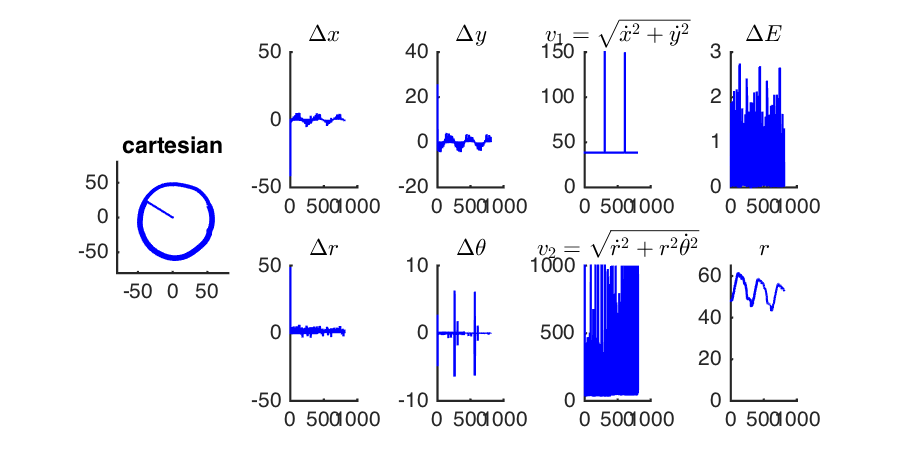
\includegraphics[bb=0 0 432 216,width=1\columnwidth]{gcodesim.png}
    \caption{Numerical computation of screw speed}
    \label{fig:noise}
\end{figure}

(\ref{eq:controller})式による制御結果
Figure \ref{fig:noise}を見ると,下段$v_2$で示されるスクリュー速度が振動していることが読み取れる.これを適当なローパスフィルターで除去することを考える.

\paragraph{FIRフィルタ}
阻止域減衰量60dBとして,窓関数法でローパスフィルタを設計する.
カイザー窓は以下で与えられる.
\begin{eqnarray*}
	w(n) = \frac{I_0 \left( \alpha \sqrt{1-\left(\frac{2n}{N-1}\right)^2} \right) }{I_0(\alpha)}	
\end{eqnarray*}
ただし,$I_0({\alpha})$は0次の第1種変形ベッセル関数
\begin{eqnarray*}
 I_0(z)	= \sum_{k=0}^{\infty}\frac{\left(\frac{z^2}{4}\right)}{k!\Gamma (k+1)}
\end{eqnarray*}
であり,$\Gamma$はガンマ関数$\Gamma(z) = \int_0^{\infty} t^{z-1}e^{-t} dt$である.

$\alpha = 6.0$として,以下の2種類のローパスフィルタを設計する.

\begin{tabular}{crr}
\toprule
FIRフィルタ  & No.1 & No.2 \\
\midrule
通過域端周波数 $\omega_p$[rad] & $0.4 \pi$ & $0.005 \pi$ \\
阻止域端周波数 $\omega_s$[rad] & $0.6 \pi$ & $0.01 \pi$ \\
フィルタ段数 & 39 & 1521 \\
\bottomrule
\end{tabular}


フィルタ段数はカイザー窓の遷移帯域幅に関するテーブルを参照して求めた.これらのFIRフィルタのインパルス応答と正規化振幅特性$H(e^{j \omega})$を Figure \ref{eq:fir_window},Figure \ref{eq:fir_window2}に示す.


\begin{figure}[htbp]
    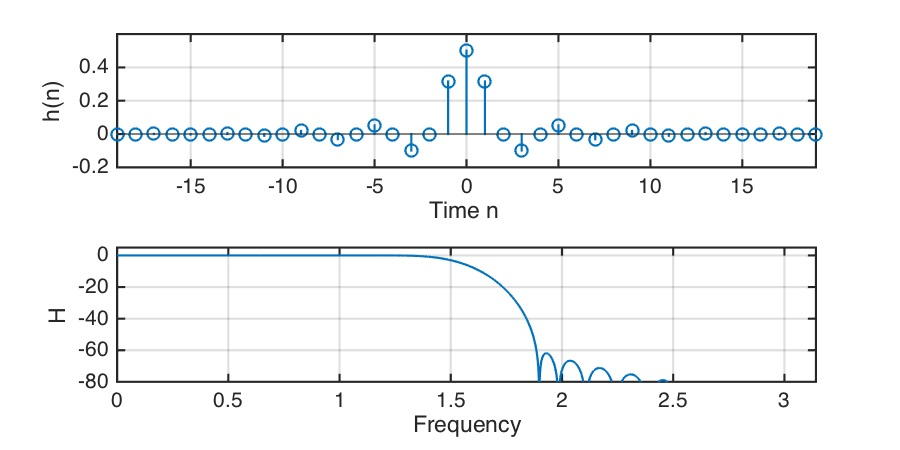
\includegraphics[bb=0 0 432 216,width=1\columnwidth]{impulse_h.pdf}
    \caption{FIR filter No.1 with kaiser window function}
   \label{eq:fir_window}
\end{figure}

\begin{figure}[htbp]
    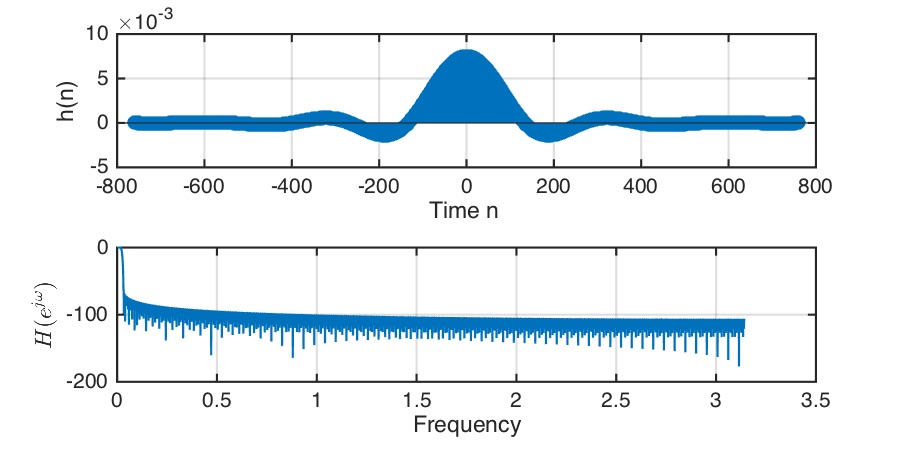
\includegraphics[bb=0 0 432 216,width=1\columnwidth]{impulse1521.pdf}
    \caption{FIR filter No.2 with kaiser window function}
   \label{eq:fir_window2}
\end{figure}

フィルタリングする前のSNW時系列データの$z$変換を$X(z)$,フィルター出力の$z$変換を$Y(z)$とすれば,フィルターの畳込みは
\begin{eqnarray*}
	Y(z) = H(z) X(z)
\end{eqnarray*}
であり,これを逆$z$変換することで時系列が求まる.
逆$z$変換は以下で求める.
\begin{eqnarray*}
	\{y_n\} = \mathcal{Z}^{-1}[(Y(z))] = \frac{1}{2 \pi i} \oint_c Y(z) z^{n-1} dz
\end{eqnarray*}

2つのFIRフィルタを用いたフィルタリング後のSNW時系列データをFigure \ref{fig:filtered}, Figure \ref{fig:filtered2}に示す.

\begin{figure}[htbp]
    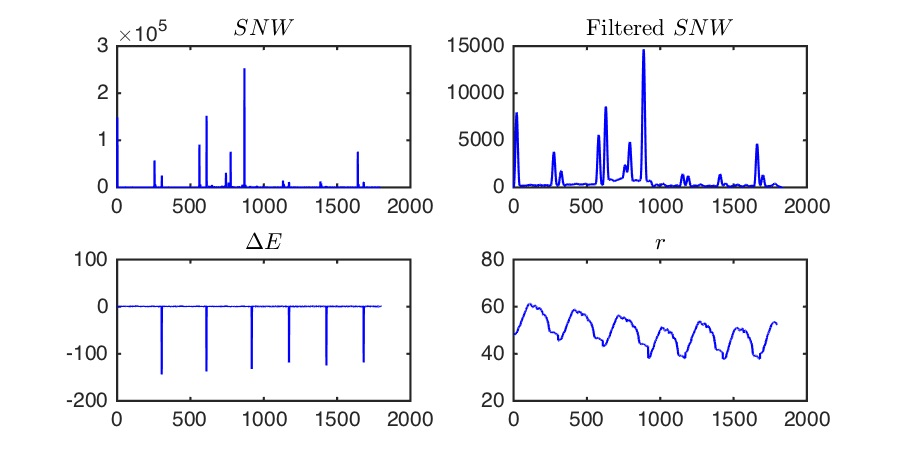
\includegraphics[bb=0 0 432 216,width=1\columnwidth]{snw_filtered.pdf}
    \caption{SNW after FIR filter No.1}
   \label{fig:filtered2}
\end{figure}

\begin{figure}[htbp]
    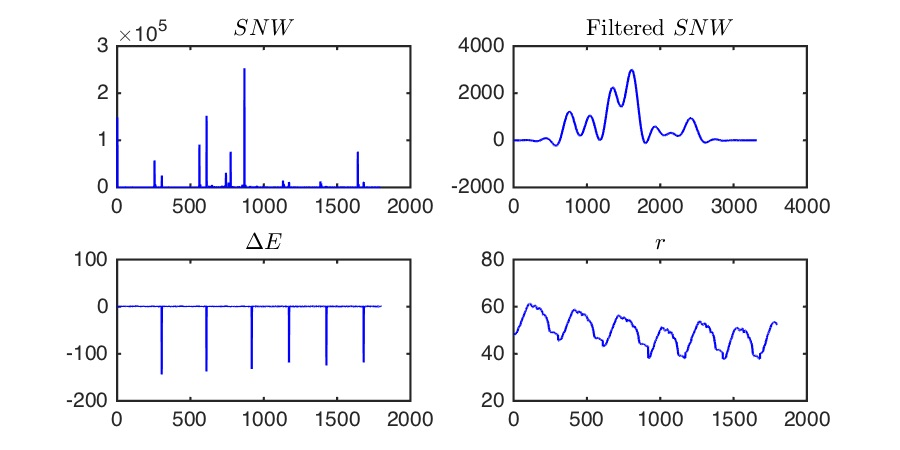
\includegraphics[bb=0 0 432 216,width=1\columnwidth]{gcodesim_filtered.pdf}
    \caption{SNW after FIR filter No.2}
   \label{fig:filtered}
\end{figure}

%\begin{figure}[htbp]
%    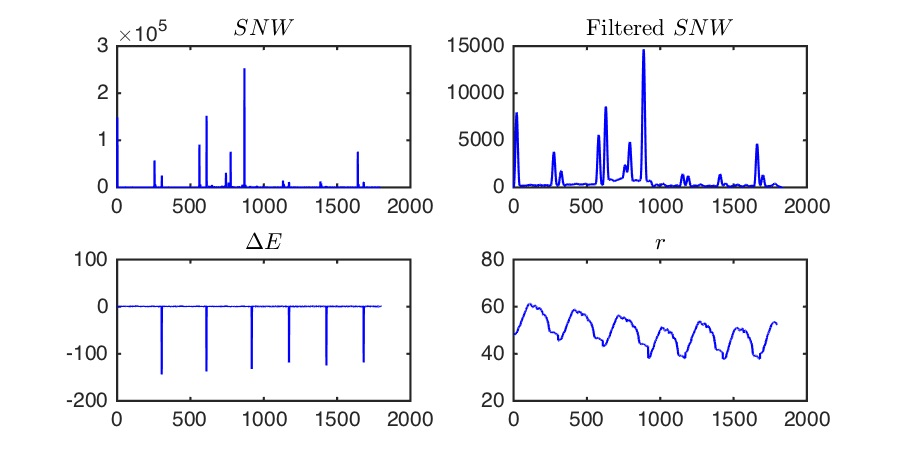
\includegraphics[bb=0 0 432 216,width=1\columnwidth]{snw_filtered.pdf}
%    \caption{SNW after FIR filtering}
%   \label{fig:filtered}
%\end{figure}

SNWの波形は原波形に比べてなまっているものの,$r$の推移に追従しているわけではない.


%\subsubsection{非線形カルマンフィルタ}
%\paragraph{拡張カルマンフィルタ(EKF)}
%(\ref{eq:controller})式を離散時間における非線形状態空間表現で表す.
%\begin{eqnarray*}\label{eq:nonlinear}
%\bm{x}(k+1) &=& \bm{f}(\bm{x}(k))+\bm{b}v(k)\\
%y(k) &=& h(\bm{x}(k))+w(k)
%\end{eqnarray*}
%
%$\bm{f}(\bm{x}), h(\bm{x})$のヤコビ行列をそれぞれ$\bm{A}(k), \bm{c}^T(k)$とおけば,
%\begin{eqnarray*}
%\bm{A}(k) &=& \frac{\partial \bm{f}(\bm{x})}{\partial \bm{x}} \bigg| _{\bm{x}=\hat{\bm{x}}(k)}\\
%\bm{c}^T(k) &=& \frac{\partial h(\bm{x})}{\partial \bm{x} } \bigg| _{\bm{x}=\hat{\bm{x}}^{-}(k)}
%\end{eqnarray*}
%
%
%このとき,(\ref{eq:nonlinear})式は
%\begin{eqnarray*}
%\bm{x}(k+1) &=& \bm{A}(k)\bm{x}(k) + \bm{b}v(k)+\bm{u}(k)\\
%z(k) &=& \bm{c}^T(k)\bm{x}(k)
%\end{eqnarray*}
%
%拡張カルマンフィルタ(EKF)のアルゴリズムは以下のように表される.
%  \begin{breakitembox}[l]{拡張カルマンフィルタ}
%    \hspace{-0.3in} $\Box$ 時間更新式\\
%    $k=1,2,...,N$に対して以下を実行\\
%     $\bullet$ 予測ステップ\\
%     事前状態推定値: \\
%     $\:\:\:\:\:\: \hat{\bm{x}}^{-}(k) = \bm{f}(\hat{\bm{x}}(k-1))$ \\
%線形近似: \\
%     $\:\:\:\:\:\: \bm{A}(k) = \frac{\partial \bm{f}(\bm{x})}{\partial \bm{x}} \bigg| _{\bm{x}=\hat{\bm{x}}(k)} $ \\
%     $\:\:\:\:\:\: \bm{c}^T(k) = \frac{\partial h(\bm{x})}{\partial \bm{x} } \bigg| _{\bm{x}=\hat{\bm{x}}^{-}(k)} $ \\
%     事前誤差共分散行列: \\
%     $\:\:\:\:\:\: \bm{P}^{-}(k) = \bm{A}(k-1)\bm{P}(k-1)\bm{A}^T(k-1) + \sigma_v^2(k-1)\bm{b}\bm{b}^T$ \\
%     $\bullet$ フィルタリングステップ\\
%     カルマンゲイン: \\
%     $\:\:\:\:\:\: \bm{g}(k)= \frac{\bm{P}^{-}(k) \bm{c}(k)}{\bm{c}^T \bm{P}^{-}(k)\bm{c}(k) + \sigma_v^2} $\\
%     状態推定値: \\
%     $\:\:\:\:\:\: \hat{\bm{x}}(k) = \hat{\bm{x}}^{-}(k) + \bm{g}(k)\{y(k)-h(\hat{x}^{-}(k))\}$\\
%     事後誤差共分散行列: \\
%     $\:\:\:\:\:\: \bm{P}^(k)=\{ \bm{I}-\bm{g}(k)\bm{c}^T(k)\} \bm{P}^{-1}(k)$
%  \end{breakitembox}
%
%ただし共分散行列$\bm{P}^{-1}(k), \bm{P}(k)$は$n \times n$行列,カルマンゲイン$\bm{G}(k)$は$n \times p$行列である.


%\paragraph{アンセンテッドカルマンフィルタ(UKF)}
%非線形関数$\bm{f}: \mathfrak{R}^n \rightarrow \mathfrak{R}^n$が$n$次元確率変数$\bm{x}$を$n$次元確率変数$\bm{y}$に変換するとき,$\bm{x}$を1次モーメント統計量と2次モーメント統計量で表現するためのシグマポイントは,スケーリングパラメータを$\kappa$とすると以下のように表される.
%\begin{eqnarray*}
%	\mathscr{X}_0 &=& \bar{\bm{x}} \\
%	\mathscr{X}_i &=& \bar{\bm{x}} + \sqrt{n+\kappa}(\sqrt{\bm{P}_x})_i\\
%	\mathscr{X}_{n+1} &=& \bar{\bm{x}} - \sqrt{n+\kappa}(\sqrt{\bm{P}_x})_i
%\end{eqnarray*}
%$\bm{P}_x$は共分散行列の定義から正定値対称行列であり,したがって$\sqrt{\bm{P}_x}$はコレスキー分解によって求まる.
%
%上のシグマポイントを用いて確率密度関数をU変換する.具体的には,
%\begin{eqnarray*}
%	\mathscr{Y}_i &=& \bm{f}(\mathscr{X}_i) \\
%	\bar{\bm{y}} &=& \sum_{i=0}^{2n} w_i \mathscr{Y}_i) \\
%	\bm{P}_y &=& \sum_{i=0}^{2n} w_i (\mathscr{Y}_i - \bar{\bm{y}}) (\mathscr{Y}_i - \bar{\bm{y}})^{T}
%\end{eqnarray*}
%
%
%アンセンテッドカルマンフィルタ(UKF)のアルゴリズムは以下のように表される.
%
%  \begin{breakitembox}[l]{UKF}
%    \hspace{-0.3in} $\Box$ 初期値\\
%    状態推定値の初期値$\hat{x}(0)$は、$N(\bm{x}_0,\bm{\Sigma}_0)$に従う正規性確率ベクトルとする。すなわち、\\
%    $\:\:\:\:\:\: \hat{\bm{x}}(0) = E[\bm{x}(0)] = \bm{x}(0)$ \\
%    $\:\:\:\:\:\: \bm{P}(0) = E[\bm{x}(0)-E[\bm{x}(0)]] = \bm{\Sigma}_0$ \\
%    $\Box$ 時間更新式\\
%    $k=1,2,...,N$に対して以下を実行\\
%     $\bullet$ シグマポイントの計算\\
%	$\:\:\:\:\:\: \mathscr{X}_0(k-1) = \bar{\bm{x}}(k-1) $\\
%	$\:\:\:\:\:\: \mathscr{X}_i(k-1) = \bar{\bm{x}}(k-1) + \sqrt{n+\kappa}(\sqrt{\bm{P}(k-1)})_i $ \\
%	$\:\:\:\:\:\: \mathscr{X}_{n+1}(k-1) = \bar{\bm{x}}(k-1) - \sqrt{n+\kappa}(\sqrt{\bm{P}(k-1)})_i $ \\
%     $\bullet$ 予測ステップ\\
%     シグマポイントの更新: \\
%	$\:\:\:\:\:\: \mathscr{X}_{i}^{-}(k) = \bm{f}(\mathscr{X}_{i}(k-1)) $ \\
%     事前状態推定値: \\
%     $\:\:\:\:\:\: \hat{\bm{x}}^{-}(k) = \sum_{i=0}^{2n} w_i \mathscr{X}^{-}(k)$\\
%     事前誤差共分散行列: \\
%     $\:\:\:\:\:\: \bm{P}^{-}(k)= \sum_{i=0}^{2n} w_i \{ \mathscr{X}_i^{-}(k) - \hat{\bm{x}}^{-}(k) \} \{ \mathscr{X}_i^{-}(k) - \hat{\bm{x}}^{-}(k) \}^T + 2\sigma_v^2 \bm{b} \bm{b}^T$ \\
%     シグマポイントの再計算: \\
%	$\:\:\:\:\:\: \mathscr{X}_0(k) = \bar{\bm{x}}(k) $\\
%	$\:\:\:\:\:\: \mathscr{X}_i(k) = \bar{\bm{x}}(k) + \sqrt{n+\kappa}(\sqrt{\bm{P}^{-}(k)})_i $ \\
%	$\:\:\:\:\:\: \mathscr{X}_{n+1}(k) = \bar{\bm{x}}(k) - \sqrt{n+\kappa}(\sqrt{\bm{P}^{-}(k)})_i $ \\
%     出力のシグマポイントの更新: \\
%     $\:\:\:\:\:\: \mathscr{Y}_i^{-}(k) = h(\mathscr{X}_i^{-}(k))$ \\
%     事前出力推定値: \\
%     $\:\:\:\:\:\: \hat{y}^{-}(k) = \sum_{i=0}^{2n} w_i \mathscr{Y}_{i}^{-} (k) $ \\
%     事前出力誤差共分散行列: \\
%     $\:\:\:\:\:\: P^{-}_{yy}(k) = \sum_{i=0}^{2n} w_i \{\mathscr{Y}_i^{-}(k) - \hat{y}^{-}(k)\}^2$ \\
%     事前状態・出力誤差共分散行列: \\
%     $\:\:\:\:\:\: \bm{P}^{-}_xy(k) = \sum_{i=0}^{2n} w_i \{ \mathscr{X}_i^{-}(k) - \hat{\bm{x}}^{-}(k)\} \{\mathscr{Y}_i^{-}(k) - \hat{y}^{-}(k)\} $ \\
%     カルマンゲイン: \\
%     $\:\:\:\:\:\: \bm{g}(k)= \frac{\bm{P}^{-}_{xy}} {P_{yy}^{-}(k) + \sigma_w^2} $\\
%     $\bullet$ フィルタリングステップ\\
%     状態推定値: \\
%     $\:\:\:\:\:\: \hat{\bm{x}}(k) = \hat{\bm{x}}^{-}(k) + \bm{g}(k)(y(k)-\hat{y}^{-}(k))$\\
%     事後誤差共分散行列: \\
%     $\:\:\:\:\:\: \bm{P}^(k)=\bm{P}^{-1}(k) - \bm{g}(k)(\bm{P}^{-}_{xy}(k))^T$
%  \end{breakitembox}


\subsection{モデルの変更}
Figure \ref{fig:noise}の計算結果で示されるような高周波成分を含む速度指令をスクリューに与えても,スクリュー内部での圧力変化にもとづく樹脂の流速の応答が遅いために樹脂の出力は追従できない.ならばいっそのことモデルを変更することを考える.

樹脂の追従速度が遅いため,速度指令は時間発展に応じてなだらかにドリフトするようなモデルが好ましい.また,定性的には動径方向の変位が大きいときに射出速度を速めるような処理が必要となる.

ここではヒューリスティックな方法として,単純に半径に比例するような成分を(\ref{eq:initial})式に加えてみる.修正後の関係式を以下に示す.

\begin{eqnarray}\label{eq:fix}
  SNW = \gamma \frac{F\cdot r\cdot  \Delta E}{\sqrt{(\Delta x)^2+(\Delta y)^2}}
\end{eqnarray}

(\ref{eq:fix})式は原点より遠い場所ほどスクリュー回転数を高めるというアドホックな方法であるが,直感的にもわかりやすく,実装も単純である.

(\ref{eq:fix})式を用いて実験を行ったところ改善が見られたので,以降はこの方法を採用する.なぜこの方法がすぐれているのか,その原因については後述する.

\section{議論}
現時点で判明している問題点として,

\begin{enumerate}
     \item そもそも吐出側を一定にしたい
     \item 原点での切り返し問題
     \item エクストルーダのOn/Offの遅延
\end{enumerate}

がある.以下でそれぞれについて考察する.

\subsection{吐出側を一定にする}
現在の計画ではG-codeに応じて吐出側,すなわちスクリューの角速度を追従させることを目的としているが,これには以下の欠点がある.

\begin{itemize}
    \item 回転数値が指令されてから実際にスクリューの回転数が変更されるまでに遅延がある
    \item スクリューの回転数が変更されたあと,射出量が追従するまでに遅延がある
     \item 吐出量の変動に応じて冷却を調節する必要があるが,冷却はリニアに効くわけではない
\end{itemize}

したがって,ステージの線速度を制御したほうがよいという結論になるが,前章で述べたように極座標において線速度を一定にすることは理論的に不可能である.

では,逆にエクストルーダが一定速度で回転しているとして,これにステージ側の線速度を追従させることは可能であろうか.極座標系での速度は$r$と$\theta$を用いて(\ref{eq:vdef})式で与えられるが,$v$を与えた場合に$\Delta r$と$\Delta \theta$は一意に決まるわけではない.
加えて前章での経験では,平方根および乗算演算に起因する数値誤差が懸念されるので,直接的に$r$と$\theta$を決定することは避けたい.

ここで発想を変えて,射出量に応じた線速度から直接$r$と$\theta$の制御量を導くのではなく,なるべくこれに近しい線速度でステージが動くように本体を制御することを考える.具体的には,以下のように問題を単純化する.

\begin{quote}
     仮定1: 半径方向の速度変化は比較的小さく,回転方向の運動が主である
\end{quote}

この仮定をおけば(\ref{eq:vdef})式は$v=r \omega$と簡素化できるから,半径に反比例するようにステージ側の回転テーブルの回転数を調節すれば,エクストルーダのスクリュー回転数に追従することができる.

仮定1の妥当性として,かりに$r$の変動量$\dot{r}$が大きかったとしてもそれは瞬間的なものであり,スクリュー回転数上昇後の樹脂吐出量の応答が低速であることを踏まえれば,この変動成分は無視できると可能性が高い.$r$の絶対量は仮定後の式でも吸収できるから,問題はないと考えられる.

じつのところ,この制御方法は(\ref{eq:fix})式でスクリュー回転数を制御する方法と双対関係にある.したがって,ここで与えた検討は(\ref{eq:fix})式の妥当性を補強している.


\subsection{原点での切り返し問題}
現在のファームウェアの実装では原点で進行方向を切返すために,原点近傍での出力に継ぎ目が見られる.これを避けるためにはファームウェアのロジックを変更する必要がある.

原点での切り返しが問題になるかどうかは造形物の形状に依存する.例えばコルセットをステージ中央に配置したときのプリントでは問題になっていない.まっすぐな円筒なども問題は発生しないが,折れ曲がった指先が原点にかかるような配置を行うと原点での切り返しが発生する.

予想では,いまの実装ではアークタンジェントの計算関数によって$\Delta \theta$の解の存在範囲が$-2 \pi \leq \theta \leq  2 \pi$に限定されているため,$\theta$が巻き戻されている可能性がある.したがって,この計算部分で連続的に$\theta$を推移させれば問題は解決する見込みである.

\subsection{エクストルーダのOn/Offの遅延}
スクリュー回転数にゼロを指定するとピンが作動して射出が止められるが,このピンが再度開いた時に樹脂が流れ出るまでに遅延が発生する.これを解決する一つの方法はG-code指令を先読みすることでこの遅延分を見込んだ開閉を行うことである.

これの実現方法には(1)G-codeを先読みする方法と,(2)エクストルーダのピン開閉時にステージ側のモーターを停めてしまう方法の2通りが考えられる.組み込みの実装としては後者のほうが簡易であったので,これを採用した.

\section{Jerkの制御について}
\subsection{極座標におけるJerk}
前章で述べたように,極座標系において一般に線速度は一定にすることができない.$\dot{r}$と$\dot{\theta}$の振る舞いはファームウェア内で加速度を設定することで操作できるが,この際の瞬発的な加速度の増加(加加速度$\dot{a}$)を{\bf Jerk}と呼んでいる.

いま,極座標で加速度制御を行ったときに線速度のプロファイルがどのような様子を描くかに興味がある.極座標系での線速度は以下の式(\ref{eq:v})から計算できる.半径方向の速度$\dot{r}$と角速度$\dot{\theta}$を適当な台形プロファイルで仮定して数値計算した結果をFigure \ref{fig:jerk}に示す.図中の右で示される$v$が極座標系における線速度である.
\begin{eqnarray}\label{eq:v}
     |v| = \sqrt{ \dot{r}^2+ r^2 \dot{\theta}^2 }
\end{eqnarray}

\begin{figure}[htbp]
    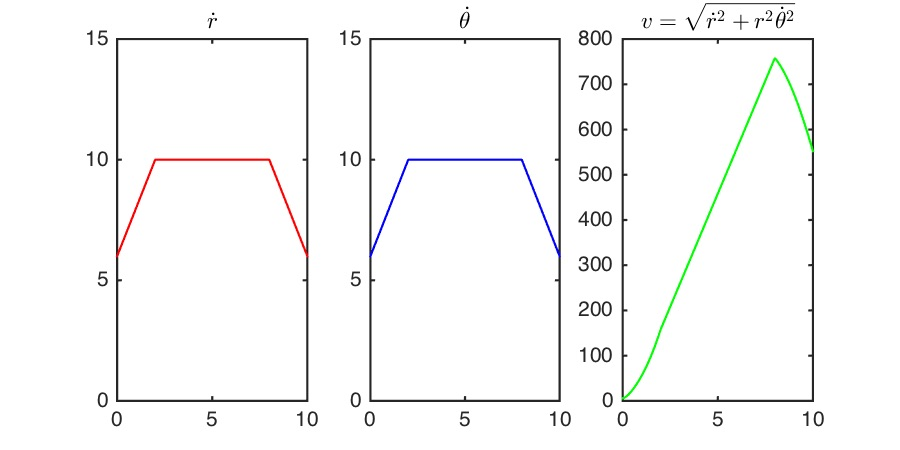
\includegraphics[bb=0 0 432 216,width=1\columnwidth]{accel2.pdf}
    \caption{Velocity profile}
    \label{fig:jerk}
\end{figure}

Figure \ref{fig:jerk}から,$\dot{r}$と$\dot{\theta}$を台形型の速度プロファイルで制御したとしても,線速度は台形型とならないことがわかる.これはデカルト座標系との違いである.

\subsection{Jerkの実装}
現在使用しているR360用のファームウェア\footnote{https://github.com/kory75/Marlin\_360}においては,前章で述べたような台形型の加減速プロファイルが実装されており,Jerkの値は初期速度(回転数)の固定値として以下のように与える.
{\small
\begin{verbatim}
#define DEFAULT_XYJERK 20.0 // (mm/sec)
#define DEFAULT_ZJERK  0.4  // (mm/sec)
#define DEFAULT_EJERK  5.0  // (mm/sec)
\end{verbatim}}

\subsection{ステージ側Jerk計算の修正}
現在の危機構成ではサーボアンプに対する指令をパルスで与えるのではなく,RS-232Cシリアル通信上のASCII文字列で指定しているため,エクストルーダのスクリュー回転数の加減速を細やかに制御するのは難しい.また,そもそもエクストルーダからの樹脂の射出の応答は遅い.

では,いっそのことステージ側の加減速計算を台形型ではなく,エクストルーダの応答に沿う形にしてはどうかという案が考えられる.しかし,そもそもJerkの制御が最終出力物の精度にどの程度影響をあたえるかという疑問が浮かぶ.

いま,問題は以下の2つに分解される.

\begin{enumerate}
     \item スライサーからのエクストルーダの値を使った場合,ステージ側の加速度はどのように制御すればよいか
     \item ステージ側のJerkを制御できたとして,それが出力物の精度に与える影響はいかほどか    
\end{enumerate}

以下で,上記の2点について考察する.

\subsubsection{ステージ側の加速度制御}
スライサーが吐き出したG-codeに記述されたエクストルーダの値から,スクリューの速度プロファイルを逆算する.いま,(\ref{eq:v})式に従って$v$が推移するとき,$\dot{r}$と$\dot{\theta}$は一意に決定できない.ここで独立変数を減らすために,$\theta$は今までと同じように線形加速制御を行うとする.いま, この$\theta$の計算に乗算器と加算器のみでステッピングモーターのパルス遅延時間を高速に計算するアルゴリズムである{\it leib ramp}\cite{leib}をすると仮定する\footnote{Marlinでも実装されている.}.

$\theta$の計算方法について詳しく述べる.
総加速ステップを$S$,ステッピングモーターの初期速度を$v_0$,目標速度を$v$,1秒ごとの加速ステップ数を$a$,加速時間を$t$とすれば,

\begin{eqnarray}\label{eq:first}
     S &=& v_0 t + \frac{1}{2} a t^2 \nonumber \\
     v &=& v_0 + a t    
\end{eqnarray}
(\ref{eq:first})における両式より,以下を得る.
\begin{eqnarray}\label{eq:second}
     S &=& \frac{v^2-v_0}{2 a} \nonumber \\
     v &=& \sqrt{v_0^2+2aS}
\end{eqnarray}
(\ref{eq:second})における両式を再帰的に適用して漸化式を導けば,
\begin{eqnarray}\label{eq:third}
     v_i = \sqrt{v_{i-1}^2 + 2a}
\end{eqnarray}
$i$ステップにおけるステッピングモーターの遅延時間を$p_i$,プロセッサのタイマー割り込み周波数を$F$とするとき,
\begin{eqnarray*}
     p_i = \frac{F}{v_i}
\end{eqnarray*}
であるから,(\ref{eq:third})式を用いることで,$p$に関する漸化式は以下のように変形できる.
\begin{eqnarray}\label{eq:fourth}
     p_i = \frac{F}{\sqrt{{(\frac{F}{p_{i-1}})}^2+2a}}
\end{eqnarray}
目標速度における遅延時間を$p_s$,定数$R= a/F^2$とおき,(\ref{eq:fourth})式をテイラー展開して1次の項で打ち切れば,
\begin{eqnarray}\label{eq:pupdate}
     p_{i+1} = p_i \cdot (1 + m \cdot p_i \cdot p_i)
\end{eqnarray}
ただし,mは以下で定義する.
\begin{eqnarray}\label{eq:mdef}
\left\{
\begin{array}{r@{\,}c@{\,}r@{\,}c@{\,}l@{\;\;}r}
 m &=& -R &:& \:\:\: \mbox{\small during acceleration}\\
 m &=& 0 &:&  \:\:\: \mbox{\small slew speed}\\
 m &=& R &:&  \:\:\: \mbox{\small during deceleration}
\end{array}%
\right.
\end{eqnarray}

(\ref{eq:mdef})式をアルゴリズムとして整理したものをAlgorithm 2に示す.

\begin{algorithm}[h]        
\begin{algorithmic}                 
\STATE $v_0, v, a, F$ given.
\STATE $S \Leftarrow (v^2-{v_0}^2) / 2 a$
\STATE $p_1 \Leftarrow F / ({v_0}^2 + 2a)^{-\frac{1}{2}}$
\STATE $p_s \Leftarrow F/v$
\STATE $R \Leftarrow a / F^2$
\STATE $T_s$ given.
\FOR{$i$ from $1$ to $T_s$}
\IF{$i \leq S$}
  \STATE $m \Leftarrow -R$
\ELSIF{$i \leq T_s-S$}
  \STATE $m \Leftarrow 0$
\ELSE
  \STATE $m \Leftarrow R$
\ENDIF
\STATE $p_{i+1} \Leftarrow p_i \cdot (1+m\cdot p \cdot p)$
\ENDFOR
\end{algorithmic}
\caption{Leib ramp acceleration}
\label{fig:leib_algorithm}                         
\end{algorithm}

これをもとに数値計算を行った例をFigure \ref{fig:leib_ramp_result}に示す.

\begin{figure}[h]
    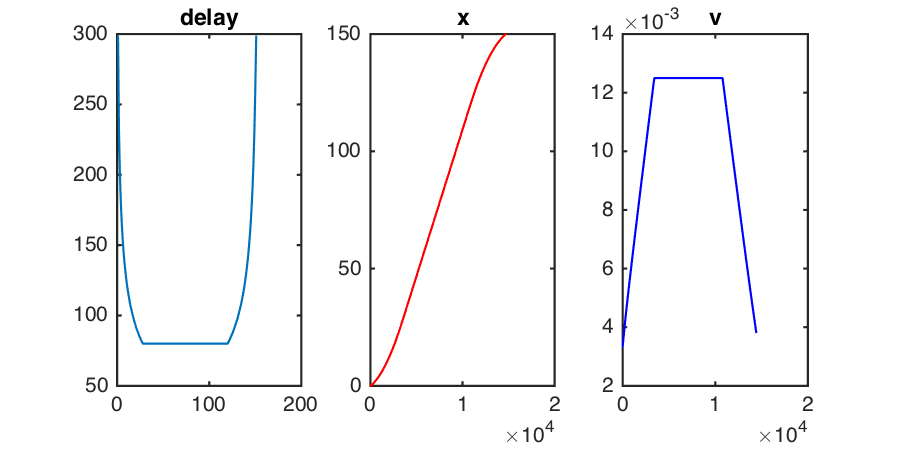
\includegraphics[bb=0 0 432 216,width=1\columnwidth]{leib_ramp_screenshot.png}
    \caption{Compute $\dot{\theta}$ with leib ramp}
    \label{fig:leib_ramp_result}
\end{figure}

いま,ある時刻における$\dot{\theta_i}$はleib rampで求まった.次に,$\dot r$は(\ref{eq:vdef})式を用いて

\begin{eqnarray}
     \bigg|\frac{dr}{dt}\bigg| = \sqrt{\frac{\Delta E}{\Delta t} - r^2 \cdot \dot \theta}
\end{eqnarray}

と表されるから,$\dot r$を求めるアルゴリズムをまとめると,Algorithm \ref{alg:drdt}のようになる.

\begin{algorithm}[h]                 
\begin{algorithmic}                 
\label{alg:drdt}                         
\STATE $\Delta E \Leftarrow E_2-E_1$
\STATE $\Delta S \Leftarrow ((x_2-x_1)^2 + (y_2-y_1)^2)^{\frac{1}{2}}$
\STATE $\Delta \theta \Leftarrow \tan^{-1} (y_2/x_2) - \tan^{-1} (y_1/x_1)$
\STATE $T_s = \alpha \cdot \Delta \theta$
\STATE compute $p_i$ with Leib Ramp.
\STATE $\dot \theta \Leftarrow 1 / p_i $
\STATE $dr/dt \Leftarrow (\Delta E/\Delta t-r^2 \cdot \dot \theta)^{\frac{1}{2}}$
\end{algorithmic}
\caption{$\dot r$ solver}
\end{algorithm}

Algorithm \ref{alg:drdt}を用いて数値計算を行った結果をFigure \ref{eq:rdot_simulation}に示す.

\begin{figure}[h]
    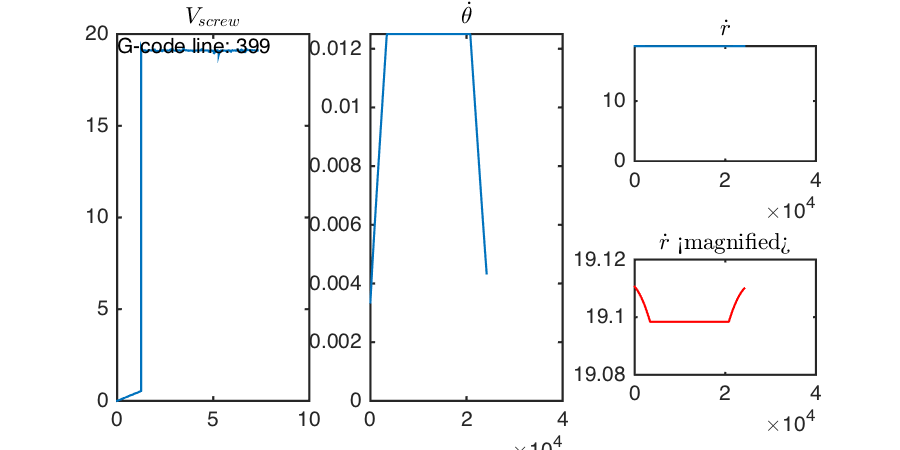
\includegraphics[bb=0 0 432 216,width=1\columnwidth]{compute_rdot_screenshot.png}
    \caption{Computed $\dot r$}
   \label{eq:rdot_simulation}
\end{figure}

\subsection{出力物の精度に与える影響の見積もり}
Figure \ref{eq:rdot_simulation}によれば,$\dot{\theta}$を線形制御した時の$\dot r$の変動は非常に小さいものである.($\sim 1.0 \times 10^{-4}$)

この結果から、$\dot r$の加速部における変動が理想的制御を行った際のx-y変位量にもたらす影響は極めて小さいと考えられる。



\begin{thebibliography}{99}
   \bibitem{rikougaku} 水島二郎,柳瀬眞一郎,理工学のための数値計算法,数理工学社 (2009)
  \bibitem{joshiki} 伊理正夫,藤野和建,『数値計算の常識』,共立出版 (1985)
   \bibitem{nagai} 永井清,土橋宏規,『ロボット機構学』,コロナ社 (2015)
    \bibitem{wakariyasui} 松日楽信人,大明準治,『わかりやすいロボットシステム入門』,オーム社 (2010)
    \bibitem{seimitsu} 松原厚,『精密位置決め・送り系設計のための制御工学』,森北出版 (2008)
  \bibitem{leib} Aryeh Eiderman, "Real Time Stepper Motor Linear Ramping Just by Addition and Multiplication," http://hwml.com/LeibRamp.pdf
   \bibitem{matlab_dsp} 川又政征,MATLABで学ぶディジタル信号処理の基礎,信号処理学会誌 (2001)
   \bibitem{scilab_dsp} 三谷政昭,Scilabで学ぶディジタル信号処理,CQ出版 (2006)
\end{thebibliography}


\end{document}
